\documentclass{standalone}
\usepackage{tikz}
\usetikzlibrary{patterns, positioning}

\begin{document}
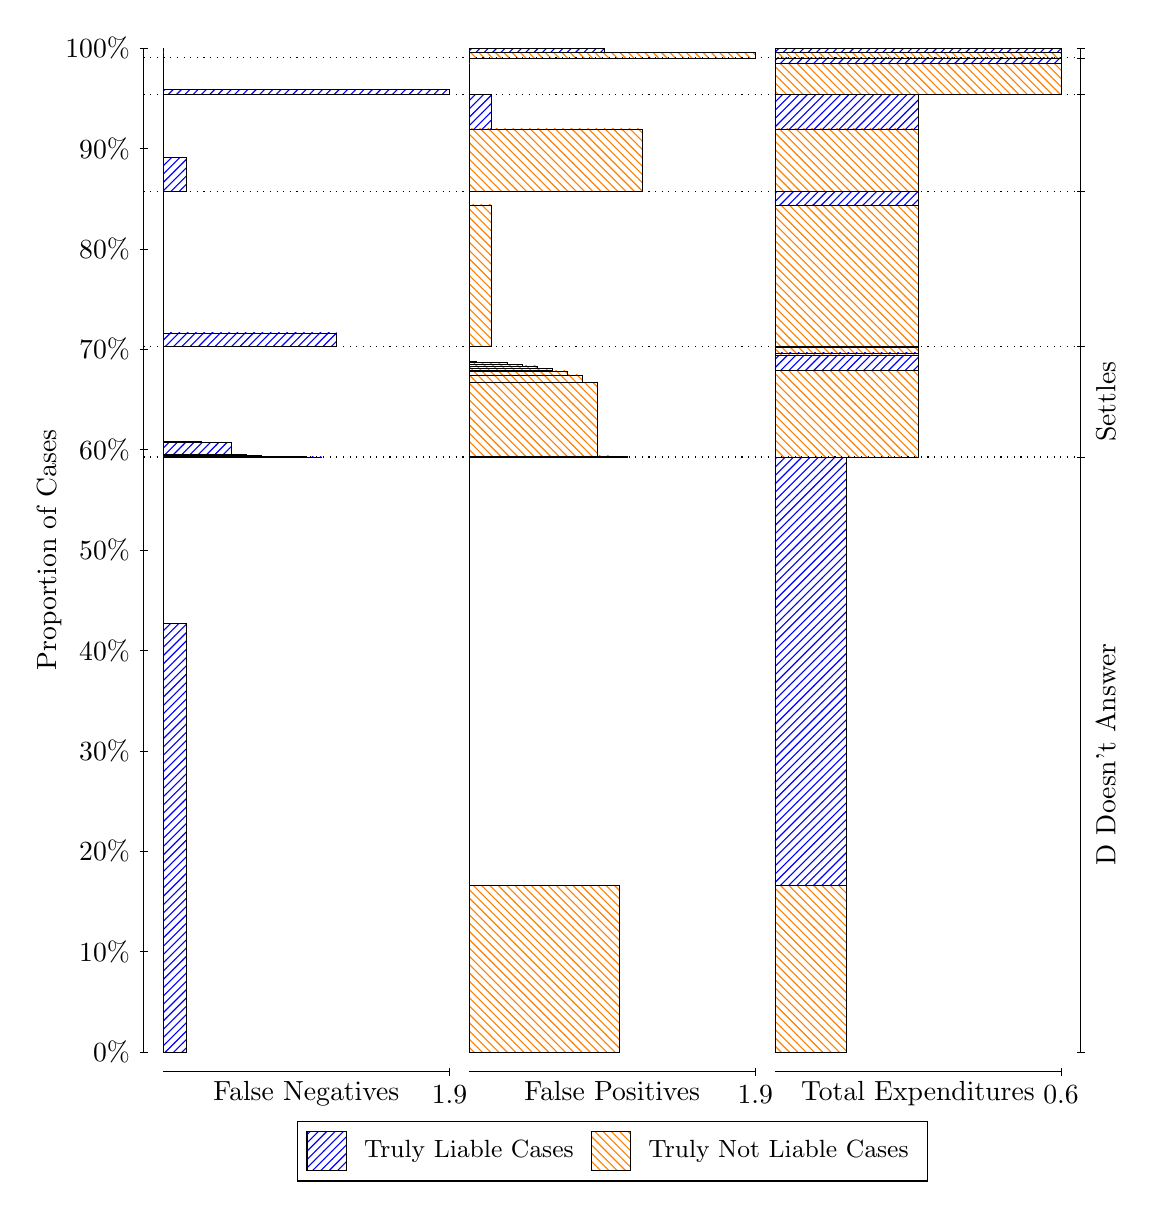
\begin{tikzpicture}
\draw[black, very thin] (1.5,1.75) -- (1.5,14.5);
\node[rotate=90, anchor=center] at (0.3, 8.125) {Proportion of Cases};
\draw[black, very thin] (1.45,1.75) -- (1.55,1.75);
\node[anchor=east] at (1.45, 1.75) {0\%};
\draw[black, very thin] (1.45,3.025) -- (1.55,3.025);
\node[anchor=east] at (1.45, 3.025) {10\%};
\draw[black, very thin] (1.45,4.3) -- (1.55,4.3);
\node[anchor=east] at (1.45, 4.3) {20\%};
\draw[black, very thin] (1.45,5.575) -- (1.55,5.575);
\node[anchor=east] at (1.45, 5.575) {30\%};
\draw[black, very thin] (1.45,6.85) -- (1.55,6.85);
\node[anchor=east] at (1.45, 6.85) {40\%};
\draw[black, very thin] (1.45,8.125) -- (1.55,8.125);
\node[anchor=east] at (1.45, 8.125) {50\%};
\draw[black, very thin] (1.45,9.4) -- (1.55,9.4);
\node[anchor=east] at (1.45, 9.4) {60\%};
\draw[black, very thin] (1.45,10.675) -- (1.55,10.675);
\node[anchor=east] at (1.45, 10.675) {70\%};
\draw[black, very thin] (1.45,11.95) -- (1.55,11.95);
\node[anchor=east] at (1.45, 11.95) {80\%};
\draw[black, very thin] (1.45,13.225) -- (1.55,13.225);
\node[anchor=east] at (1.45, 13.225) {90\%};
\draw[black, very thin] (1.45,14.5) -- (1.55,14.5);
\node[anchor=east] at (1.45, 14.5) {100\%};

\draw[black, very thin] (13.4,1.75) -- (13.4,14.5);
\draw[black, very thin] (13.35,1.75) -- (13.45,1.75);
\node[anchor=west] at (13.35, 1.75) {};
\draw[black, very thin] (13.35,9.3061) -- (13.45,9.3061);
\node[anchor=west] at (13.35, 9.3061) {};
\draw[black, very thin] (13.35,10.709) -- (13.45,10.709);
\node[anchor=west] at (13.35, 10.709) {};
\draw[black, very thin] (13.35,12.682) -- (13.45,12.682);
\node[anchor=west] at (13.35, 12.682) {};
\draw[black, very thin] (13.35,13.909) -- (13.45,13.909);
\node[anchor=west] at (13.35, 13.909) {};
\draw[black, very thin] (13.35,14.375) -- (13.45,14.375);
\node[anchor=west] at (13.35, 14.375) {};
\draw[black, very thin] (13.35,14.5) -- (13.45,14.5);
\node[anchor=west] at (13.35, 14.5) {};

\draw[black, very thin, pattern color=blue, pattern=north east lines] (1.75,1.75) rectangle (2.0368,7.1937);
\draw[black, very thin, pattern color=orange, pattern=north west lines] (1.75,7.1937) rectangle (1.75,9.3061);
\draw[black, very thin, pattern color=blue, pattern=north east lines] (1.75,9.3061) rectangle (3.7579,9.3086);
\draw[black, very thin, pattern color=blue, pattern=north east lines] (1.75,9.3086) rectangle (3.5667,9.3102);
\draw[black, very thin, pattern color=blue, pattern=north east lines] (1.75,9.3102) rectangle (3.3754,9.3126);
\draw[black, very thin, pattern color=blue, pattern=north east lines] (1.75,9.3126) rectangle (3.1842,9.3172);
\draw[black, very thin, pattern color=blue, pattern=north east lines] (1.75,9.3172) rectangle (2.993,9.3235);
\draw[black, very thin, pattern color=blue, pattern=north east lines] (1.75,9.3235) rectangle (2.8018,9.3357);
\draw[black, very thin, pattern color=blue, pattern=north east lines] (1.75,9.3357) rectangle (2.6105,9.4871);
\draw[black, very thin, pattern color=blue, pattern=north east lines] (1.75,9.4871) rectangle (2.4193,9.4896);
\draw[black, very thin, pattern color=blue, pattern=north east lines] (1.75,9.4896) rectangle (2.2281,9.5028);
\draw[black, very thin, pattern color=orange, pattern=north west lines] (1.75,9.5028) rectangle (1.75,10.709);
\draw[black, very thin, pattern color=blue, pattern=north east lines] (1.75,10.709) rectangle (3.9491,10.883);
\draw[black, very thin, pattern color=orange, pattern=north west lines] (1.75,10.883) rectangle (1.75,12.682);
\draw[black, very thin, pattern color=blue, pattern=north east lines] (1.75,12.682) rectangle (2.0368,13.116);
\draw[black, very thin, pattern color=orange, pattern=north west lines] (1.75,13.116) rectangle (1.75,13.909);
\draw[black, very thin, pattern color=blue, pattern=north east lines] (1.75,13.909) rectangle (5.3833,13.979);
\draw[black, very thin, pattern color=orange, pattern=north west lines] (1.75,13.979) rectangle (1.75,14.375);
\draw[black, very thin, pattern color=orange, pattern=north west lines] (1.75,14.375) rectangle (1.75,14.444);
\draw[black, very thin, pattern color=blue, pattern=north east lines] (1.75,14.444) rectangle (1.75,14.5);
\draw[black, very thin, pattern color=orange, pattern=north west lines] (5.6333,1.75) rectangle (7.5456,3.8624);
\draw[black, very thin, pattern color=blue, pattern=north east lines] (5.6333,3.8624) rectangle (5.6333,9.3061);
\draw[black, very thin, pattern color=orange, pattern=north west lines] (5.6333,9.3061) rectangle (7.6412,9.3141);
\draw[black, very thin, pattern color=orange, pattern=north west lines] (5.6333,9.3141) rectangle (7.45,9.321);
\draw[black, very thin, pattern color=orange, pattern=north west lines] (5.6333,9.321) rectangle (7.2588,10.251);
\draw[black, very thin, pattern color=orange, pattern=north west lines] (5.6333,10.251) rectangle (7.0675,10.348);
\draw[black, very thin, pattern color=orange, pattern=north west lines] (5.6333,10.348) rectangle (6.8763,10.4);
\draw[black, very thin, pattern color=orange, pattern=north west lines] (5.6333,10.4) rectangle (6.6851,10.407);
\draw[black, very thin, pattern color=orange, pattern=north west lines] (5.6333,10.407) rectangle (6.6851,10.436);
\draw[black, very thin, pattern color=orange, pattern=north west lines] (5.6333,10.436) rectangle (6.4939,10.462);
\draw[black, very thin, pattern color=orange, pattern=north west lines] (5.6333,10.462) rectangle (6.3026,10.479);
\draw[black, very thin, pattern color=orange, pattern=north west lines] (5.6333,10.479) rectangle (6.1114,10.512);
\draw[black, very thin, pattern color=blue, pattern=north east lines] (5.6333,10.512) rectangle (5.7289,10.525);
\draw[black, very thin, pattern color=blue, pattern=north east lines] (5.6333,10.525) rectangle (5.6333,10.709);
\draw[black, very thin, pattern color=orange, pattern=north west lines] (5.6333,10.709) rectangle (5.9202,12.508);
\draw[black, very thin, pattern color=blue, pattern=north east lines] (5.6333,12.508) rectangle (5.6333,12.682);
\draw[black, very thin, pattern color=orange, pattern=north west lines] (5.6333,12.682) rectangle (7.8325,13.474);
\draw[black, very thin, pattern color=blue, pattern=north east lines] (5.6333,13.474) rectangle (5.9202,13.909);
\draw[black, very thin, pattern color=orange, pattern=north west lines] (5.6333,13.909) rectangle (5.6333,14.305);
\draw[black, very thin, pattern color=blue, pattern=north east lines] (5.6333,14.305) rectangle (5.6333,14.375);
\draw[black, very thin, pattern color=orange, pattern=north west lines] (5.6333,14.375) rectangle (9.2667,14.444);
\draw[black, very thin, pattern color=blue, pattern=north east lines] (5.6333,14.444) rectangle (7.3544,14.5);
\draw[black, very thin, pattern color=orange, pattern=north west lines] (9.5167,1.75) rectangle (10.425,3.8624);
\draw[black, very thin, pattern color=blue, pattern=north east lines] (9.5167,3.8624) rectangle (10.425,9.3061);
\draw[black, very thin, pattern color=orange, pattern=north west lines] (9.5167,9.3061) rectangle (11.333,10.407);
\draw[black, very thin, pattern color=blue, pattern=north east lines] (9.5167,10.407) rectangle (11.333,10.593);
\draw[black, very thin, pattern color=orange, pattern=north west lines] (9.5167,10.593) rectangle (11.333,10.626);
\draw[black, very thin, pattern color=blue, pattern=north east lines] (9.5167,10.626) rectangle (11.333,10.629);
\draw[black, very thin, pattern color=orange, pattern=north west lines] (9.5167,10.629) rectangle (11.333,10.701);
\draw[black, very thin, pattern color=blue, pattern=north east lines] (9.5167,10.701) rectangle (11.333,10.709);
\draw[black, very thin, pattern color=orange, pattern=north west lines] (9.5167,10.709) rectangle (11.333,12.508);
\draw[black, very thin, pattern color=blue, pattern=north east lines] (9.5167,12.508) rectangle (11.333,12.682);
\draw[black, very thin, pattern color=orange, pattern=north west lines] (9.5167,12.682) rectangle (11.333,13.474);
\draw[black, very thin, pattern color=blue, pattern=north east lines] (9.5167,13.474) rectangle (11.333,13.909);
\draw[black, very thin, pattern color=orange, pattern=north west lines] (9.5167,13.909) rectangle (13.15,14.305);
\draw[black, very thin, pattern color=blue, pattern=north east lines] (9.5167,14.305) rectangle (13.15,14.375);
\draw[black, very thin, pattern color=orange, pattern=north west lines] (9.5167,14.375) rectangle (13.15,14.444);
\draw[black, very thin, pattern color=blue, pattern=north east lines] (9.5167,14.444) rectangle (13.15,14.5);
\draw[black, dotted] (1.5,9.3061) -- (13.4,9.3061);
\draw[black, dotted] (1.5,10.709) -- (13.4,10.709);
\draw[black, dotted] (1.5,12.682) -- (13.4,12.682);
\draw[black, dotted] (1.5,13.909) -- (13.4,13.909);
\draw[black, dotted] (1.5,14.375) -- (13.4,14.375);
\draw[black, very thin] (1.75,1.5) -- (5.3833,1.5);
\node[anchor=north] at (3.5667, 1.5) {False Negatives};
\draw[black, very thin] (5.3833,1.45) -- (5.3833,1.55);
\node[anchor=north] at (5.3833, 1.45) {1.9};

\draw[black, very thin] (5.6333,1.5) -- (9.2667,1.5);
\node[anchor=north] at (7.45, 1.5) {False Positives};
\draw[black, very thin] (9.2667,1.45) -- (9.2667,1.55);
\node[anchor=north] at (9.2667, 1.45) {1.9};

\draw[black, very thin] (9.5167,1.5) -- (13.15,1.5);
\node[anchor=north] at (11.333, 1.5) {Total Expenditures};
\draw[black, very thin] (13.15,1.45) -- (13.15,1.55);
\node[anchor=north] at (13.15, 1.45) {0.6};

\node[black, centered, rotate=90] at (13.72, 5.5281) {D Doesn't Answer};
\node[black, centered, rotate=90] at (13.72, 10.007) {Settles};





\draw (7.449999999999999,1.5) node[draw=none] (baseCoordinate) {};
\begin{scope}[align=center]
        \matrix[scale=0.5, draw=black, below=0.5cm of baseCoordinate, nodes={draw}, column sep=0.1cm]{
            \node[rectangle, draw, minimum width=0.5cm, minimum height=0.5cm, pattern=north east lines, pattern color=blue] {}; &
            \node[draw=none, font=\small] (B) {Truly Liable Cases}; &
            \node[rectangle, draw, minimum width=0.5cm, minimum height=0.5cm, pattern=north west lines, pattern color=orange] {}; &
            \node[draw=none, font=\small] (B) {Truly Not Liable Cases}; \\
            };
\end{scope}

\end{tikzpicture}
\end{document}